

\chapter*{Anhang}
\begin{landscape}
    % Hier kommt der Inhalt, den du drehen möchtest


\begin{figure}[h]
    \centering
    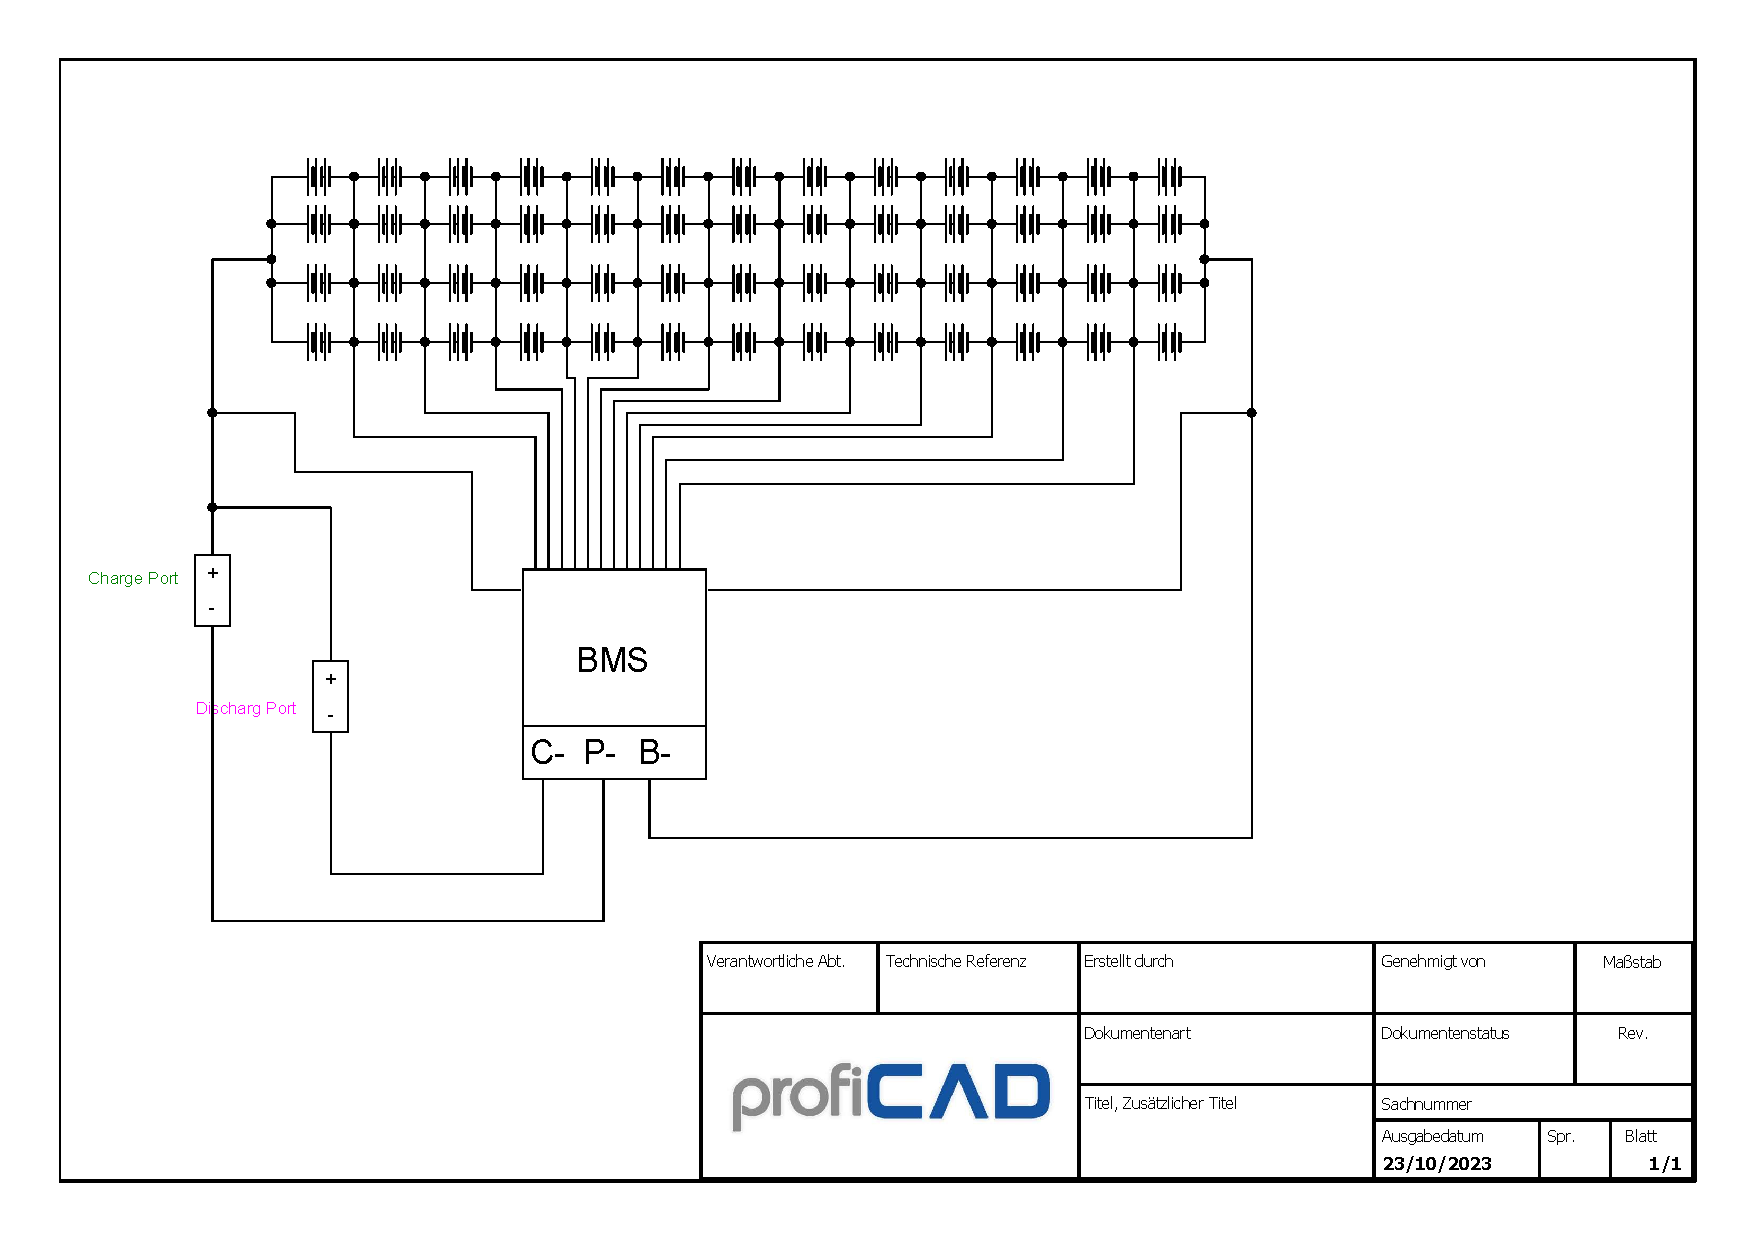
\includegraphics[width=22cm]{images/Schaltplan.pdf}
    \caption{Schaltplan\cite{lorenz_scherrer_selbst_2023}}%
    \label{fig:5_1}
\end{figure}
\end{landscape}

\begin{figure}[h]
    \centering
    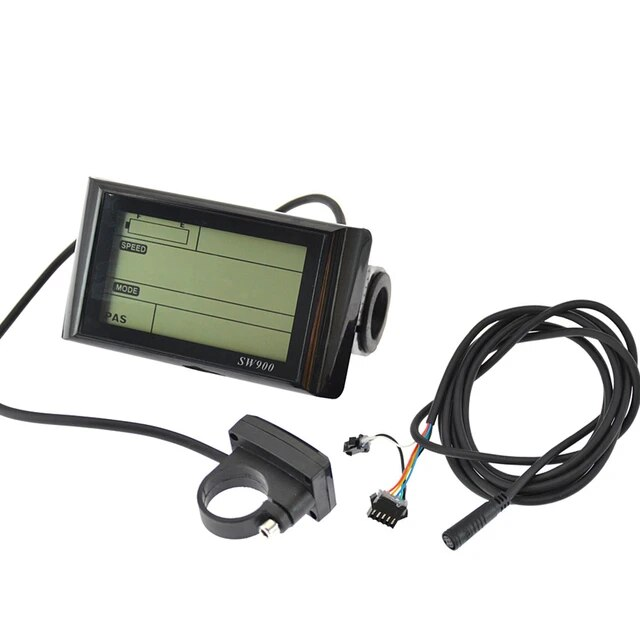
\includegraphics[width=10cm]{images/sw900.jpeg}
    \caption{sw900\cite{lorenz_scherrer_selbst_2023}}%
    \label{fig:15}
\end{figure}


\begin{figure}[h]
    \centering
    \includegraphics[width=10cm]{images/RasenmäherAkku}
    \caption{Rasenmäher Akku\cite{lorenz_scherrer_selbst_2023}}
    \label{fig:20}
\end{figure}

\begin{figure}[h]
    \centering
    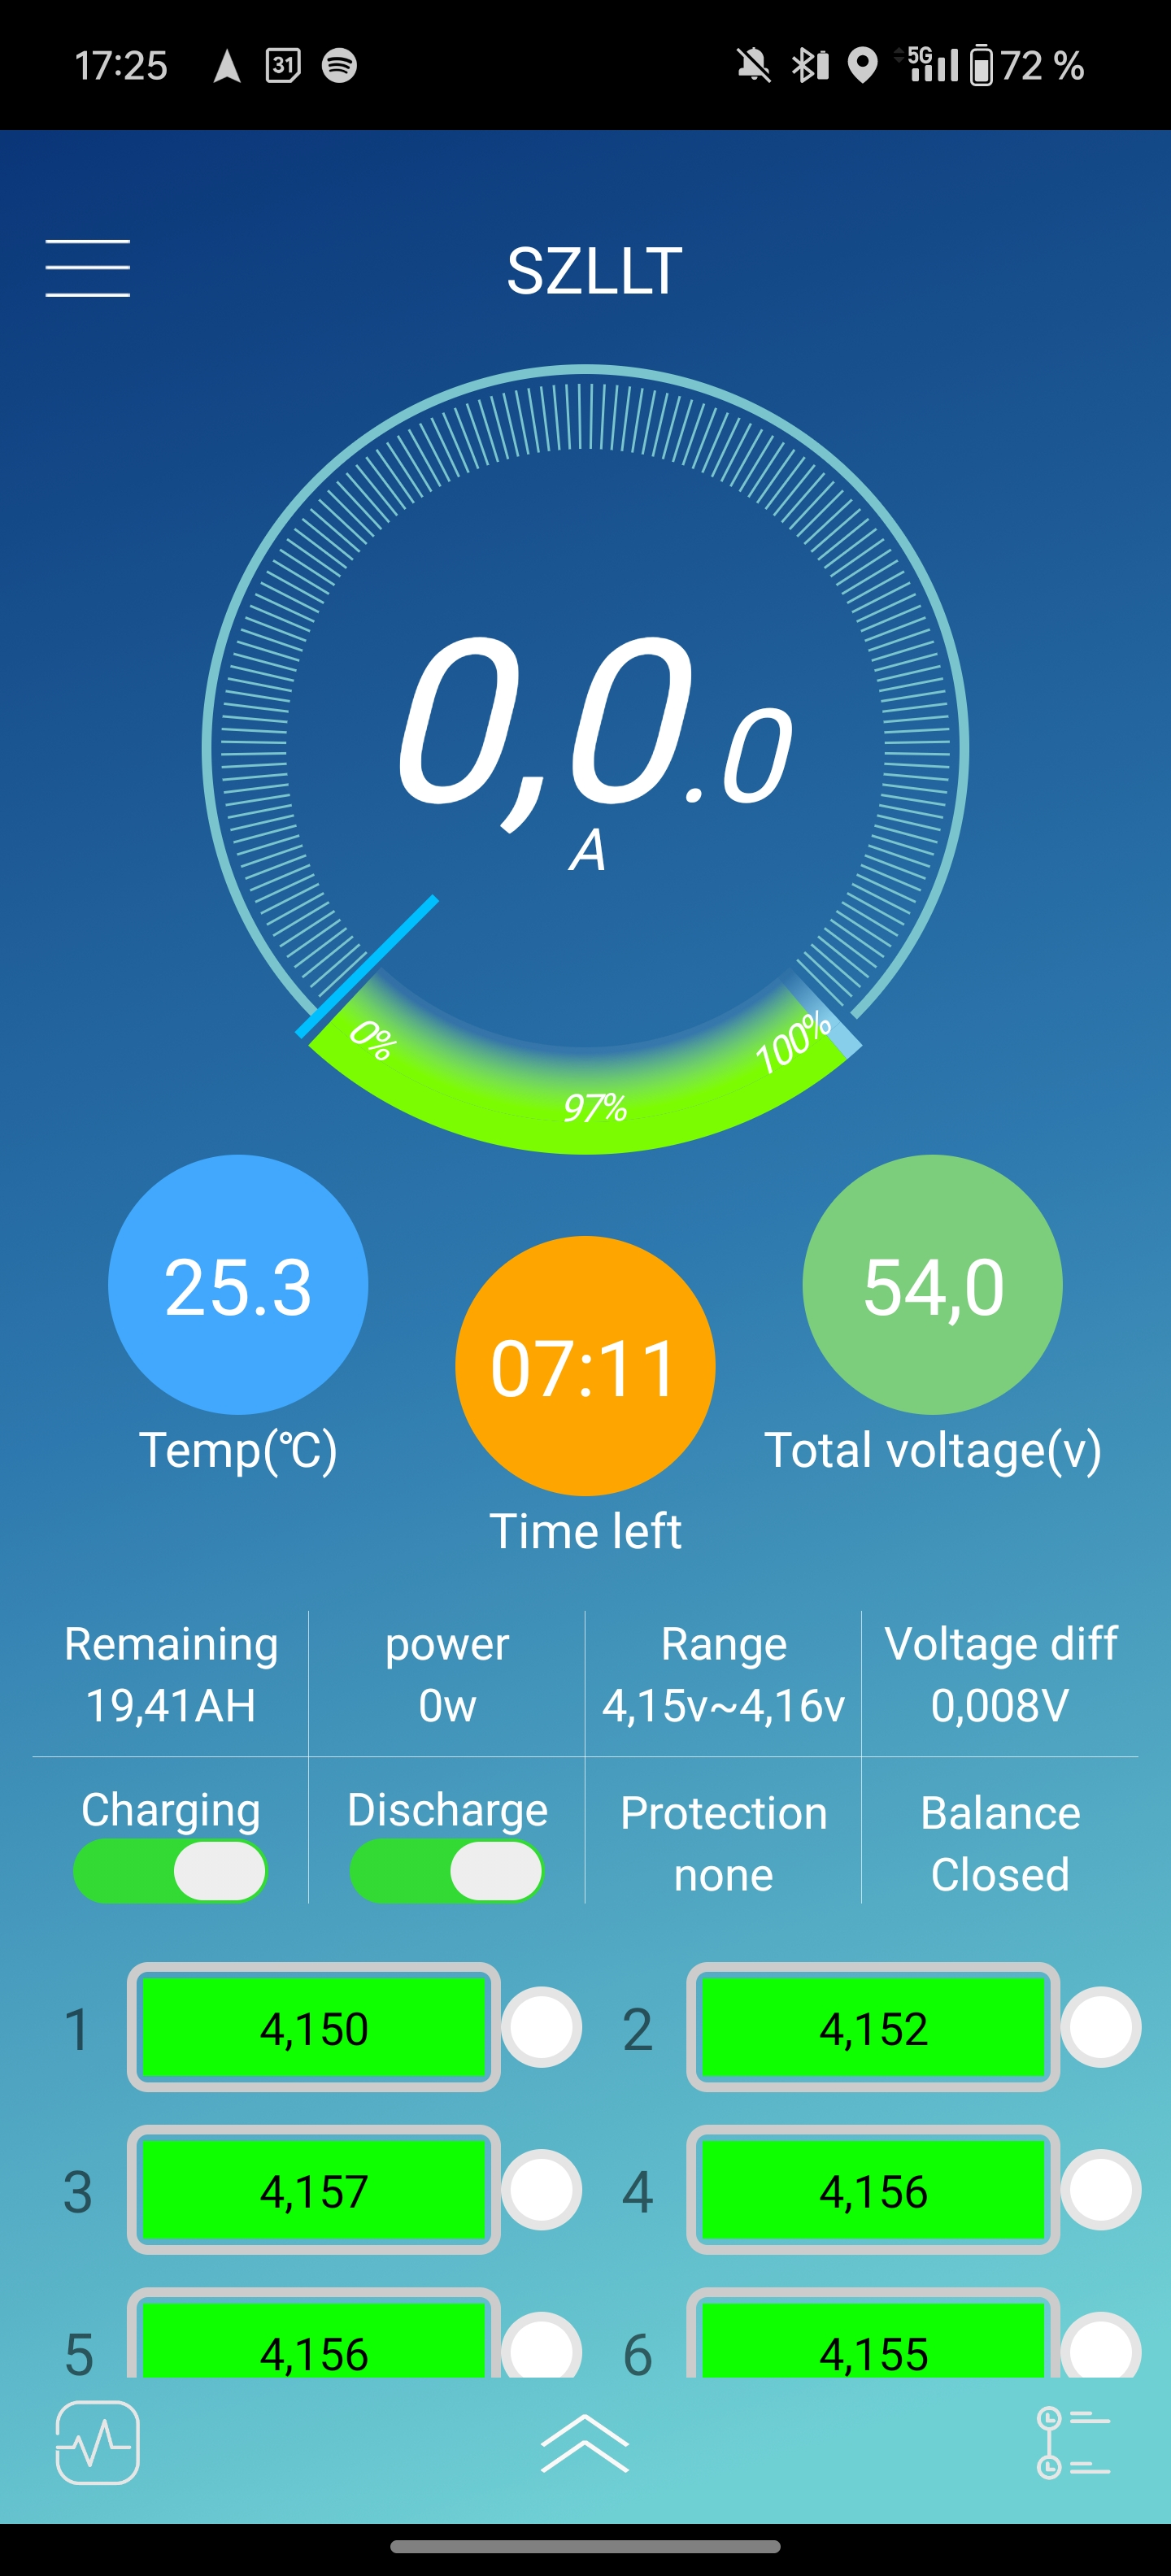
\includegraphics[width=10cm]{images/BMSvorderFahrt}
    \caption{Batterie-Stand vor der Fahrt\cite{lorenz_scherrer_selbst_2023}}
    \label{fig:31}
\end{figure}

\begin{figure}[h]
    \centering
    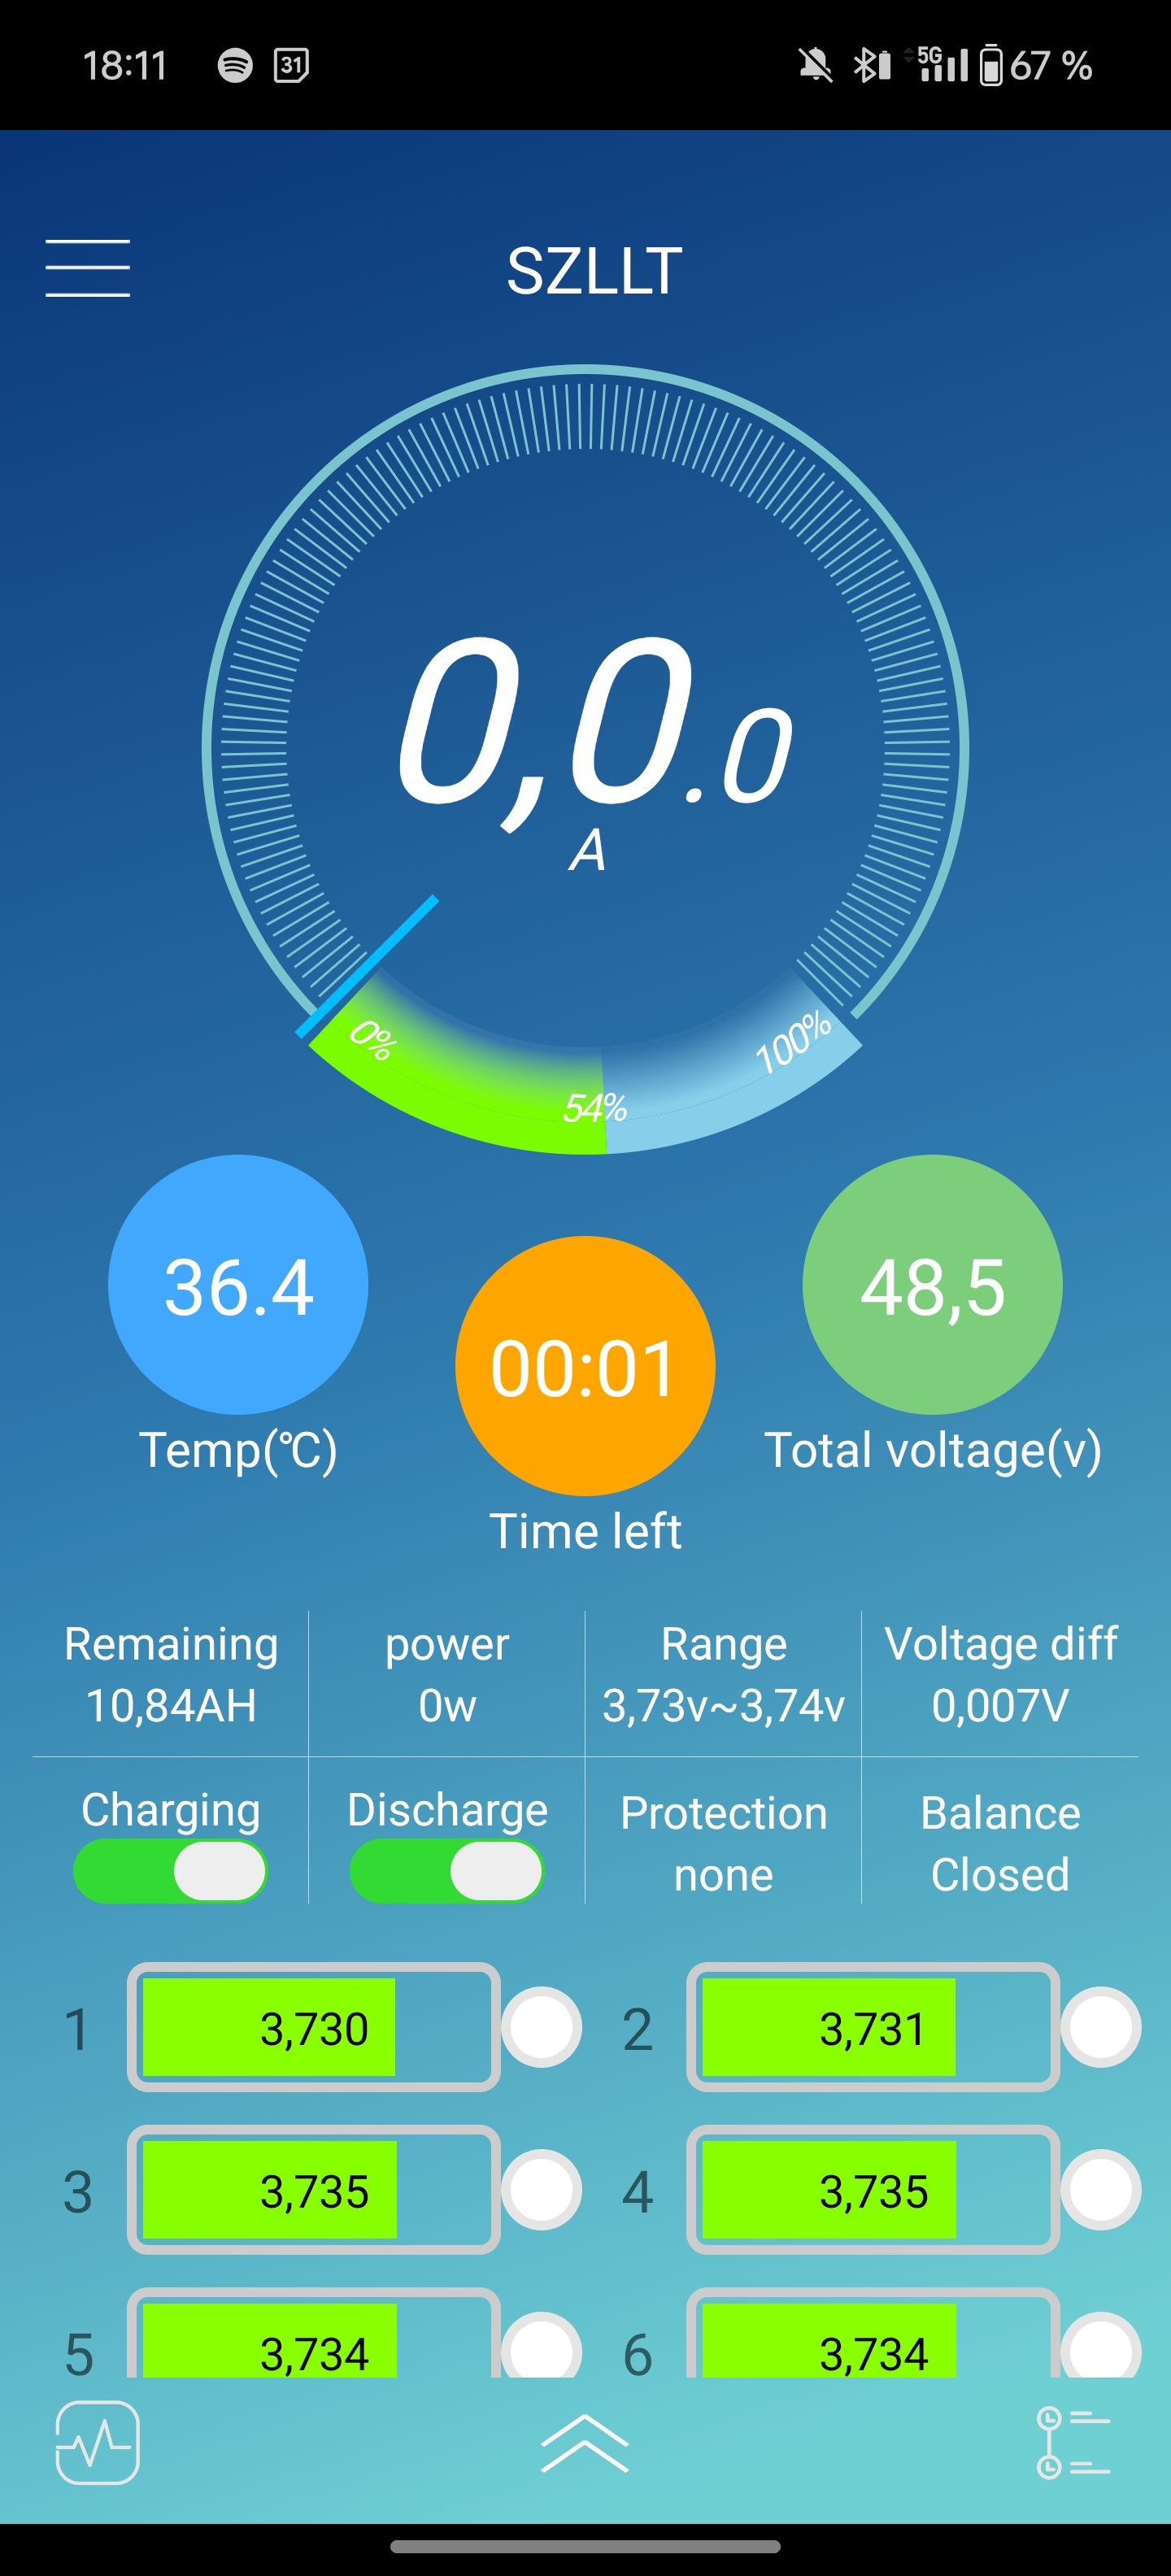
\includegraphics[width=10cm]{images/BMSnachderFahrt}
    \caption{Batterie Stand nach der Fahrt\cite{lorenz_scherrer_selbst_2023}}
    \label{fig:32}
\end{figure}

\begin{figure}[h]
    \centering
    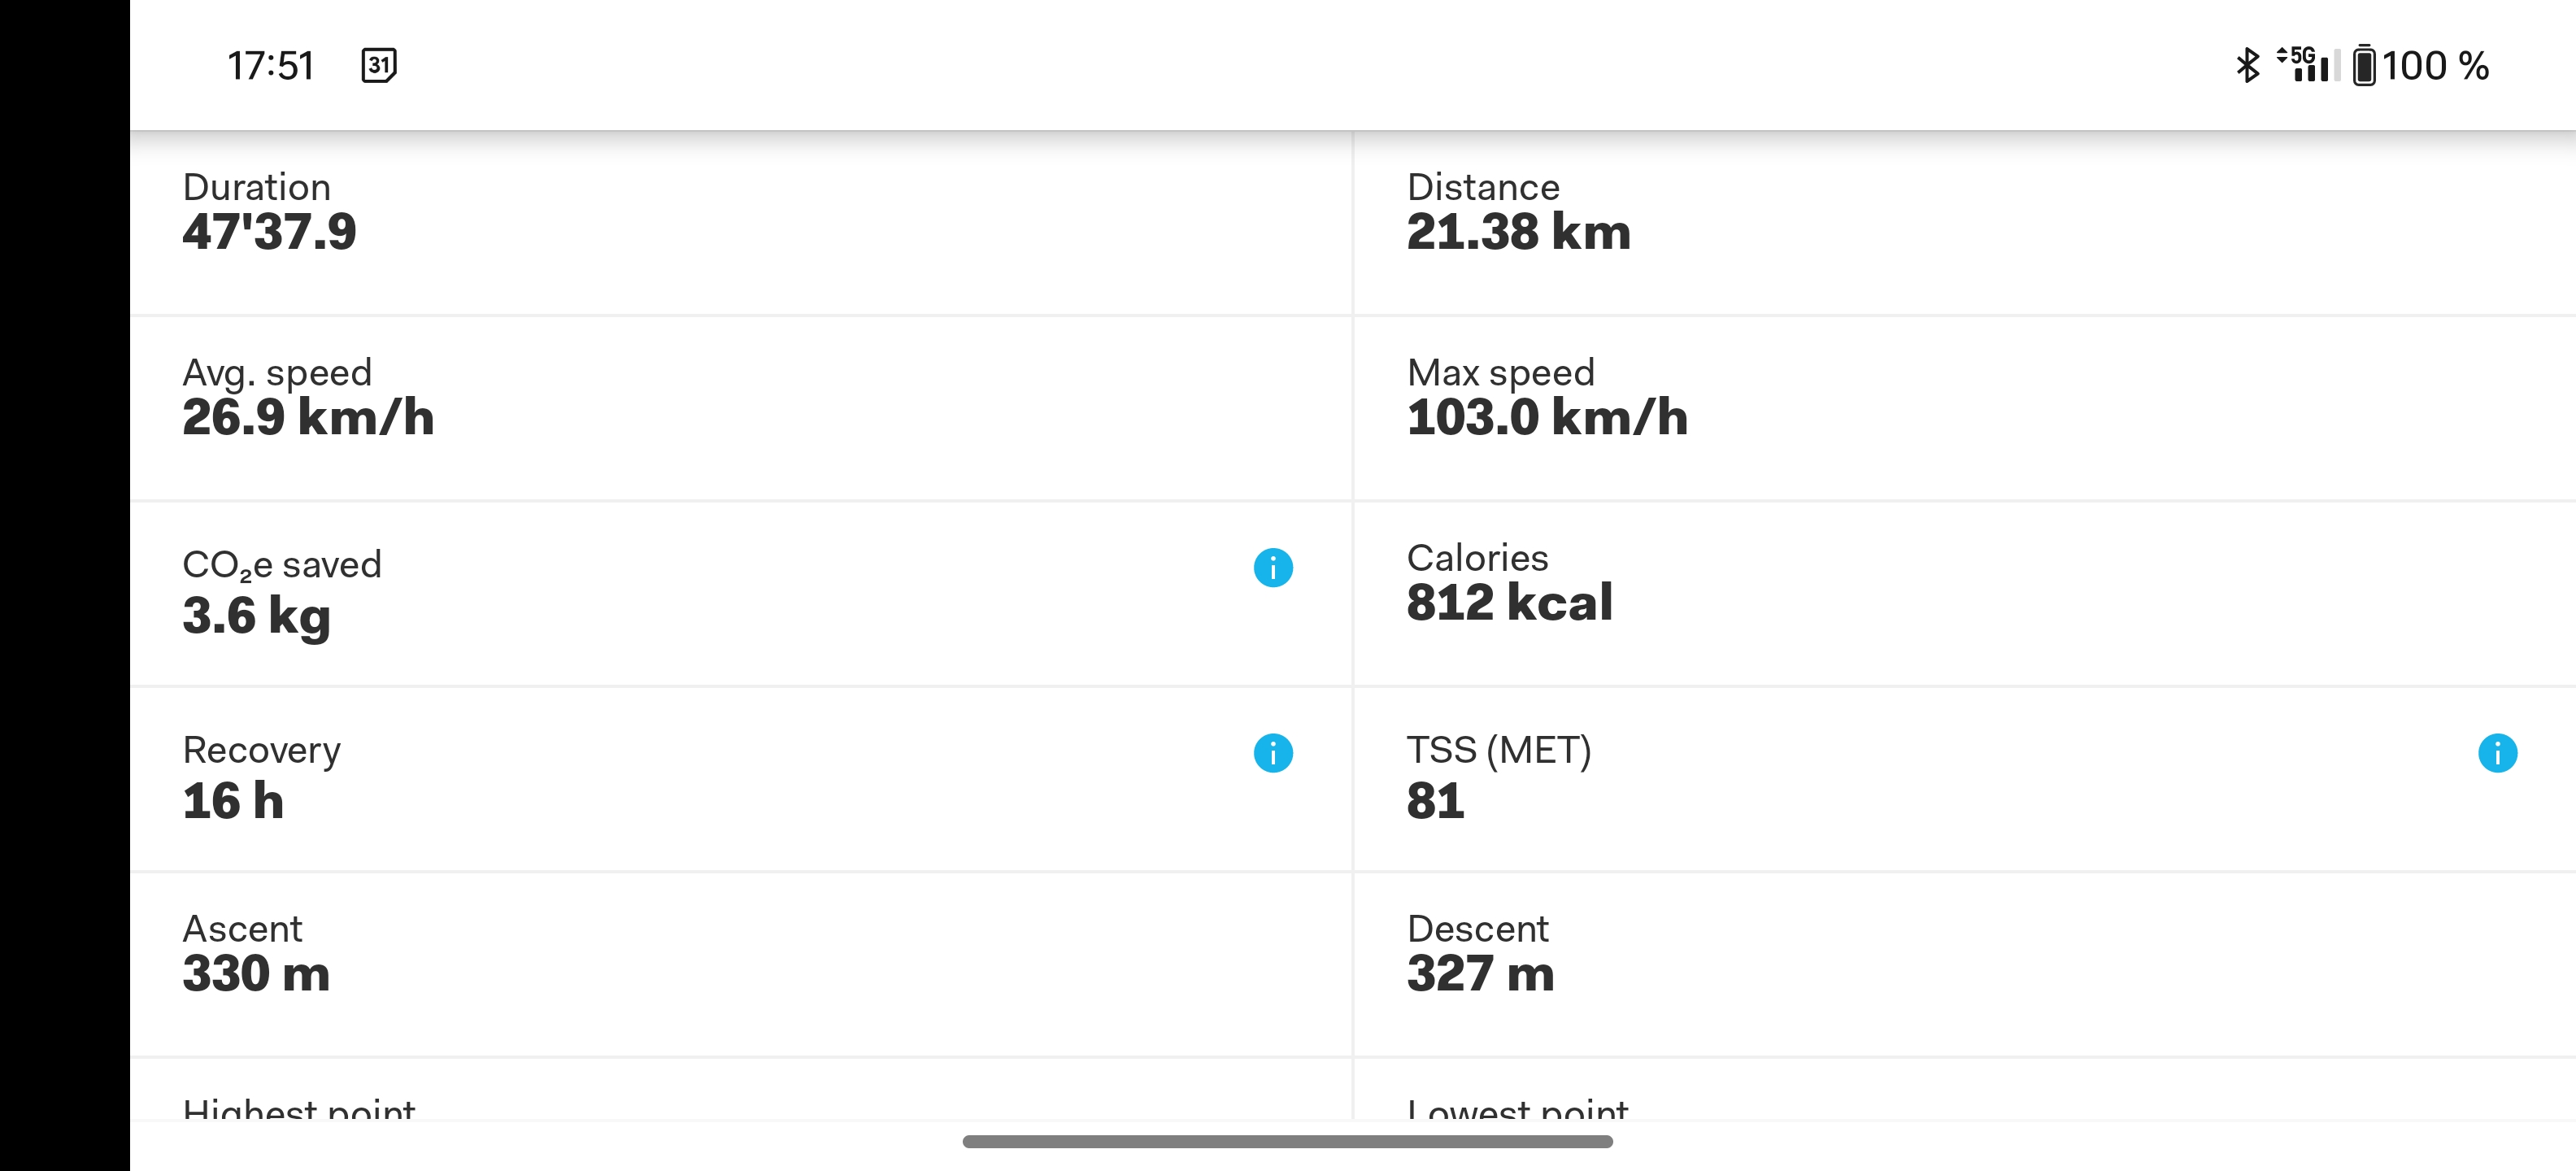
\includegraphics[width=10cm]{images/streckenparameter}
    \caption{Streckenparameter\cite{lorenz_scherrer_selbst_2023}}
    \label{fig:33}
\end{figure}

\begin{figure}[h]
    \centering
    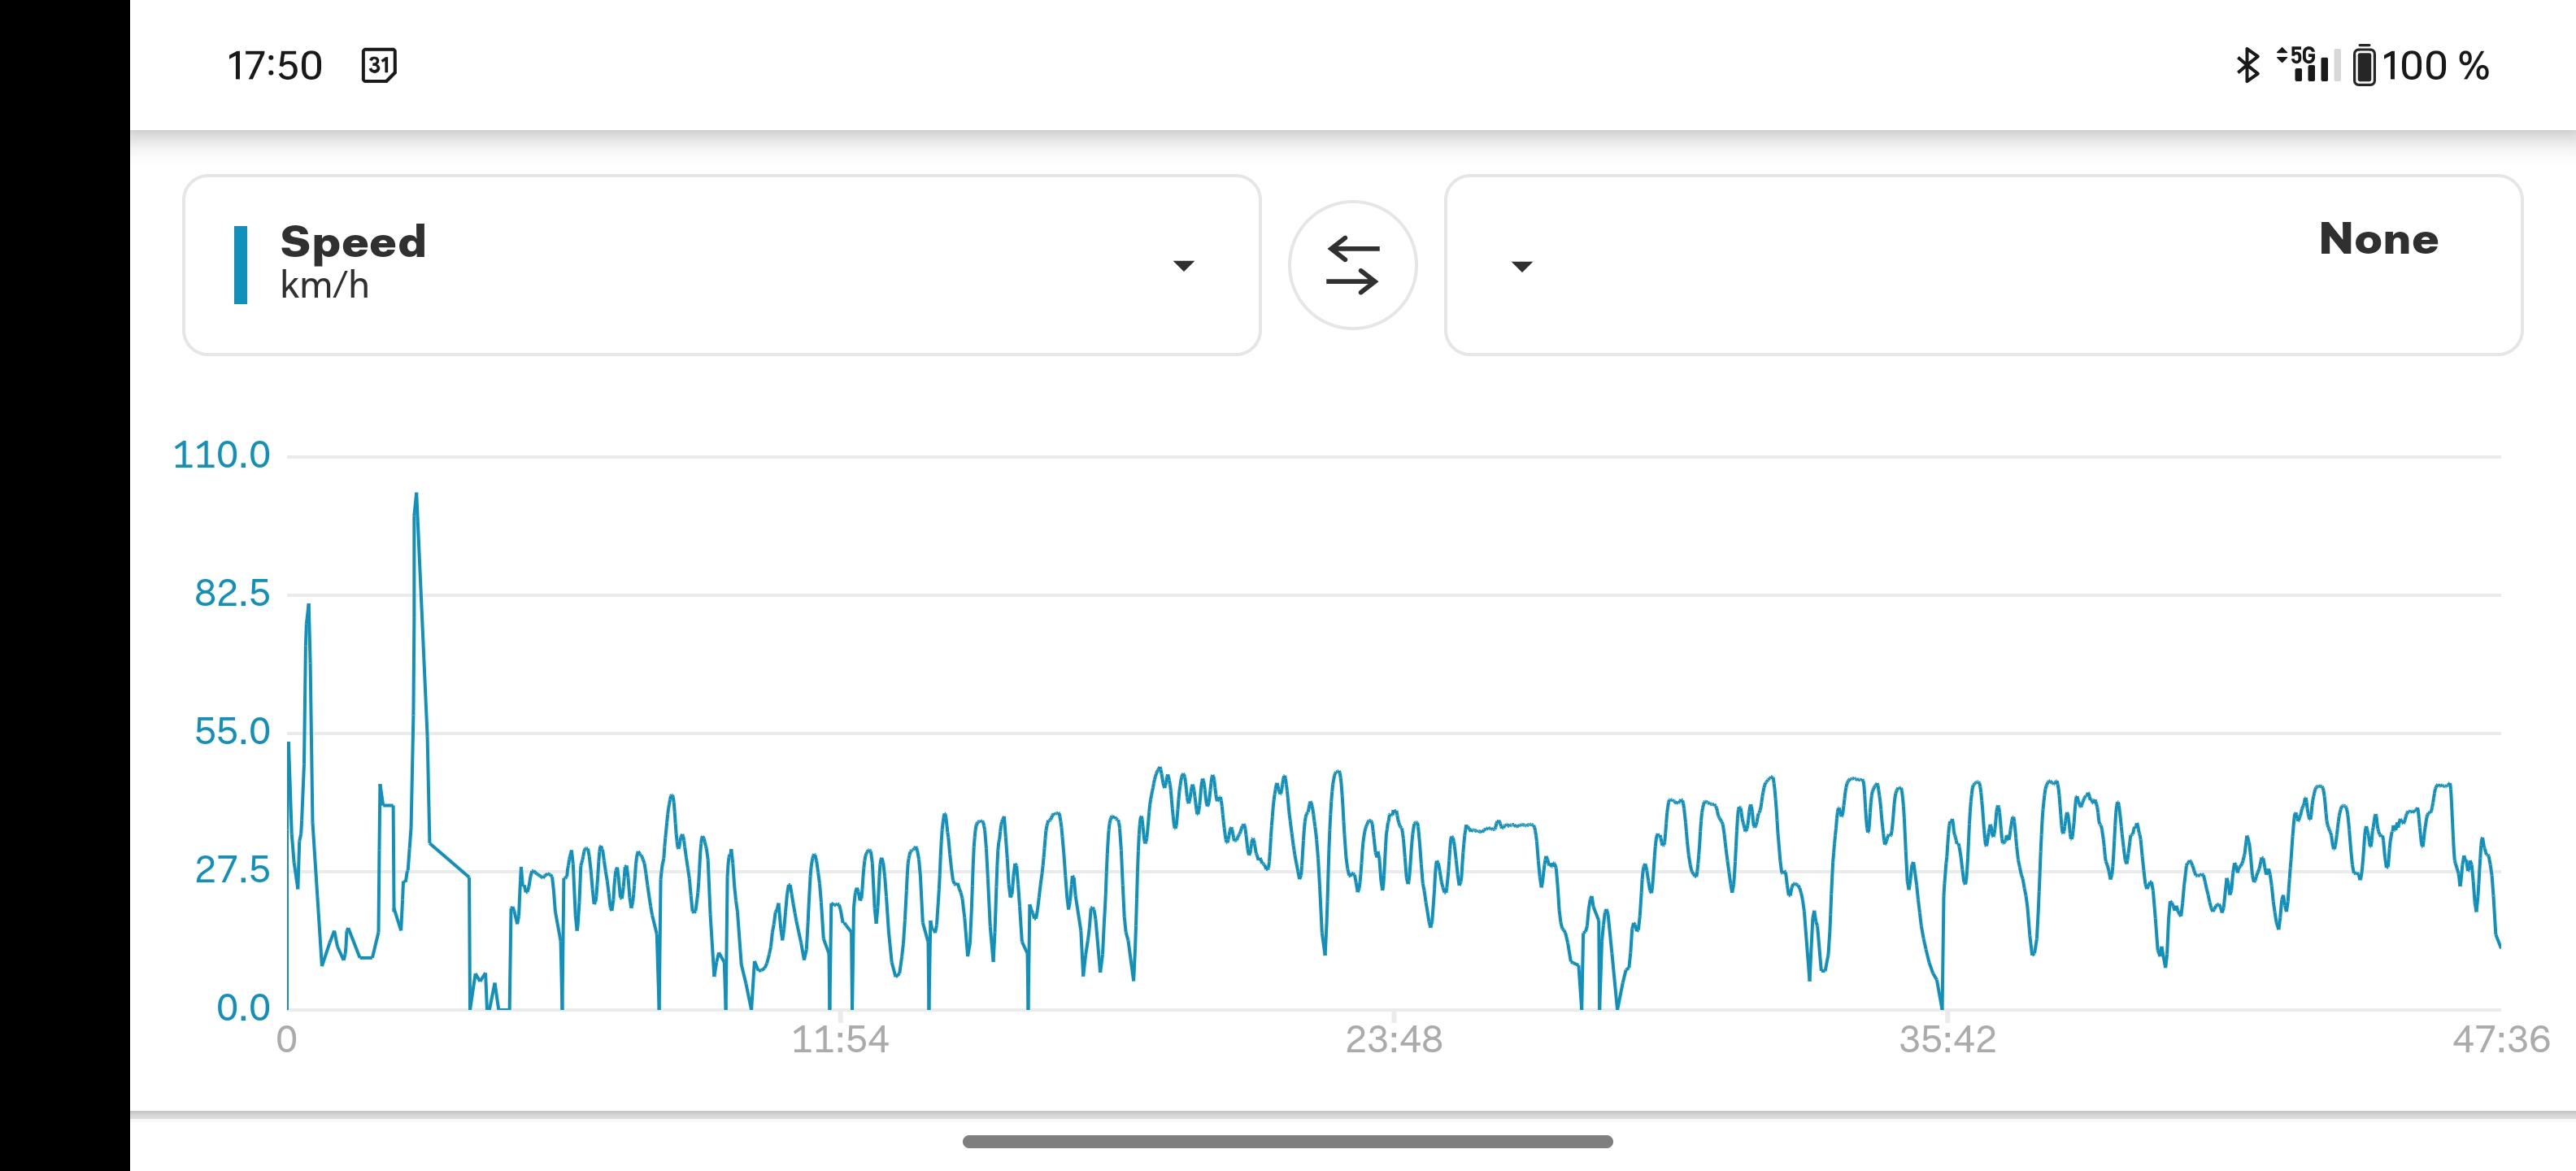
\includegraphics[width=10cm]{images/Geschwindigkeitshistogramm}
    \caption{Geschwindigkeitshistogramm\cite{lorenz_scherrer_selbst_2023}}
    \label{fig:34}
\end{figure}

\begin{figure}[h]
    \centering
    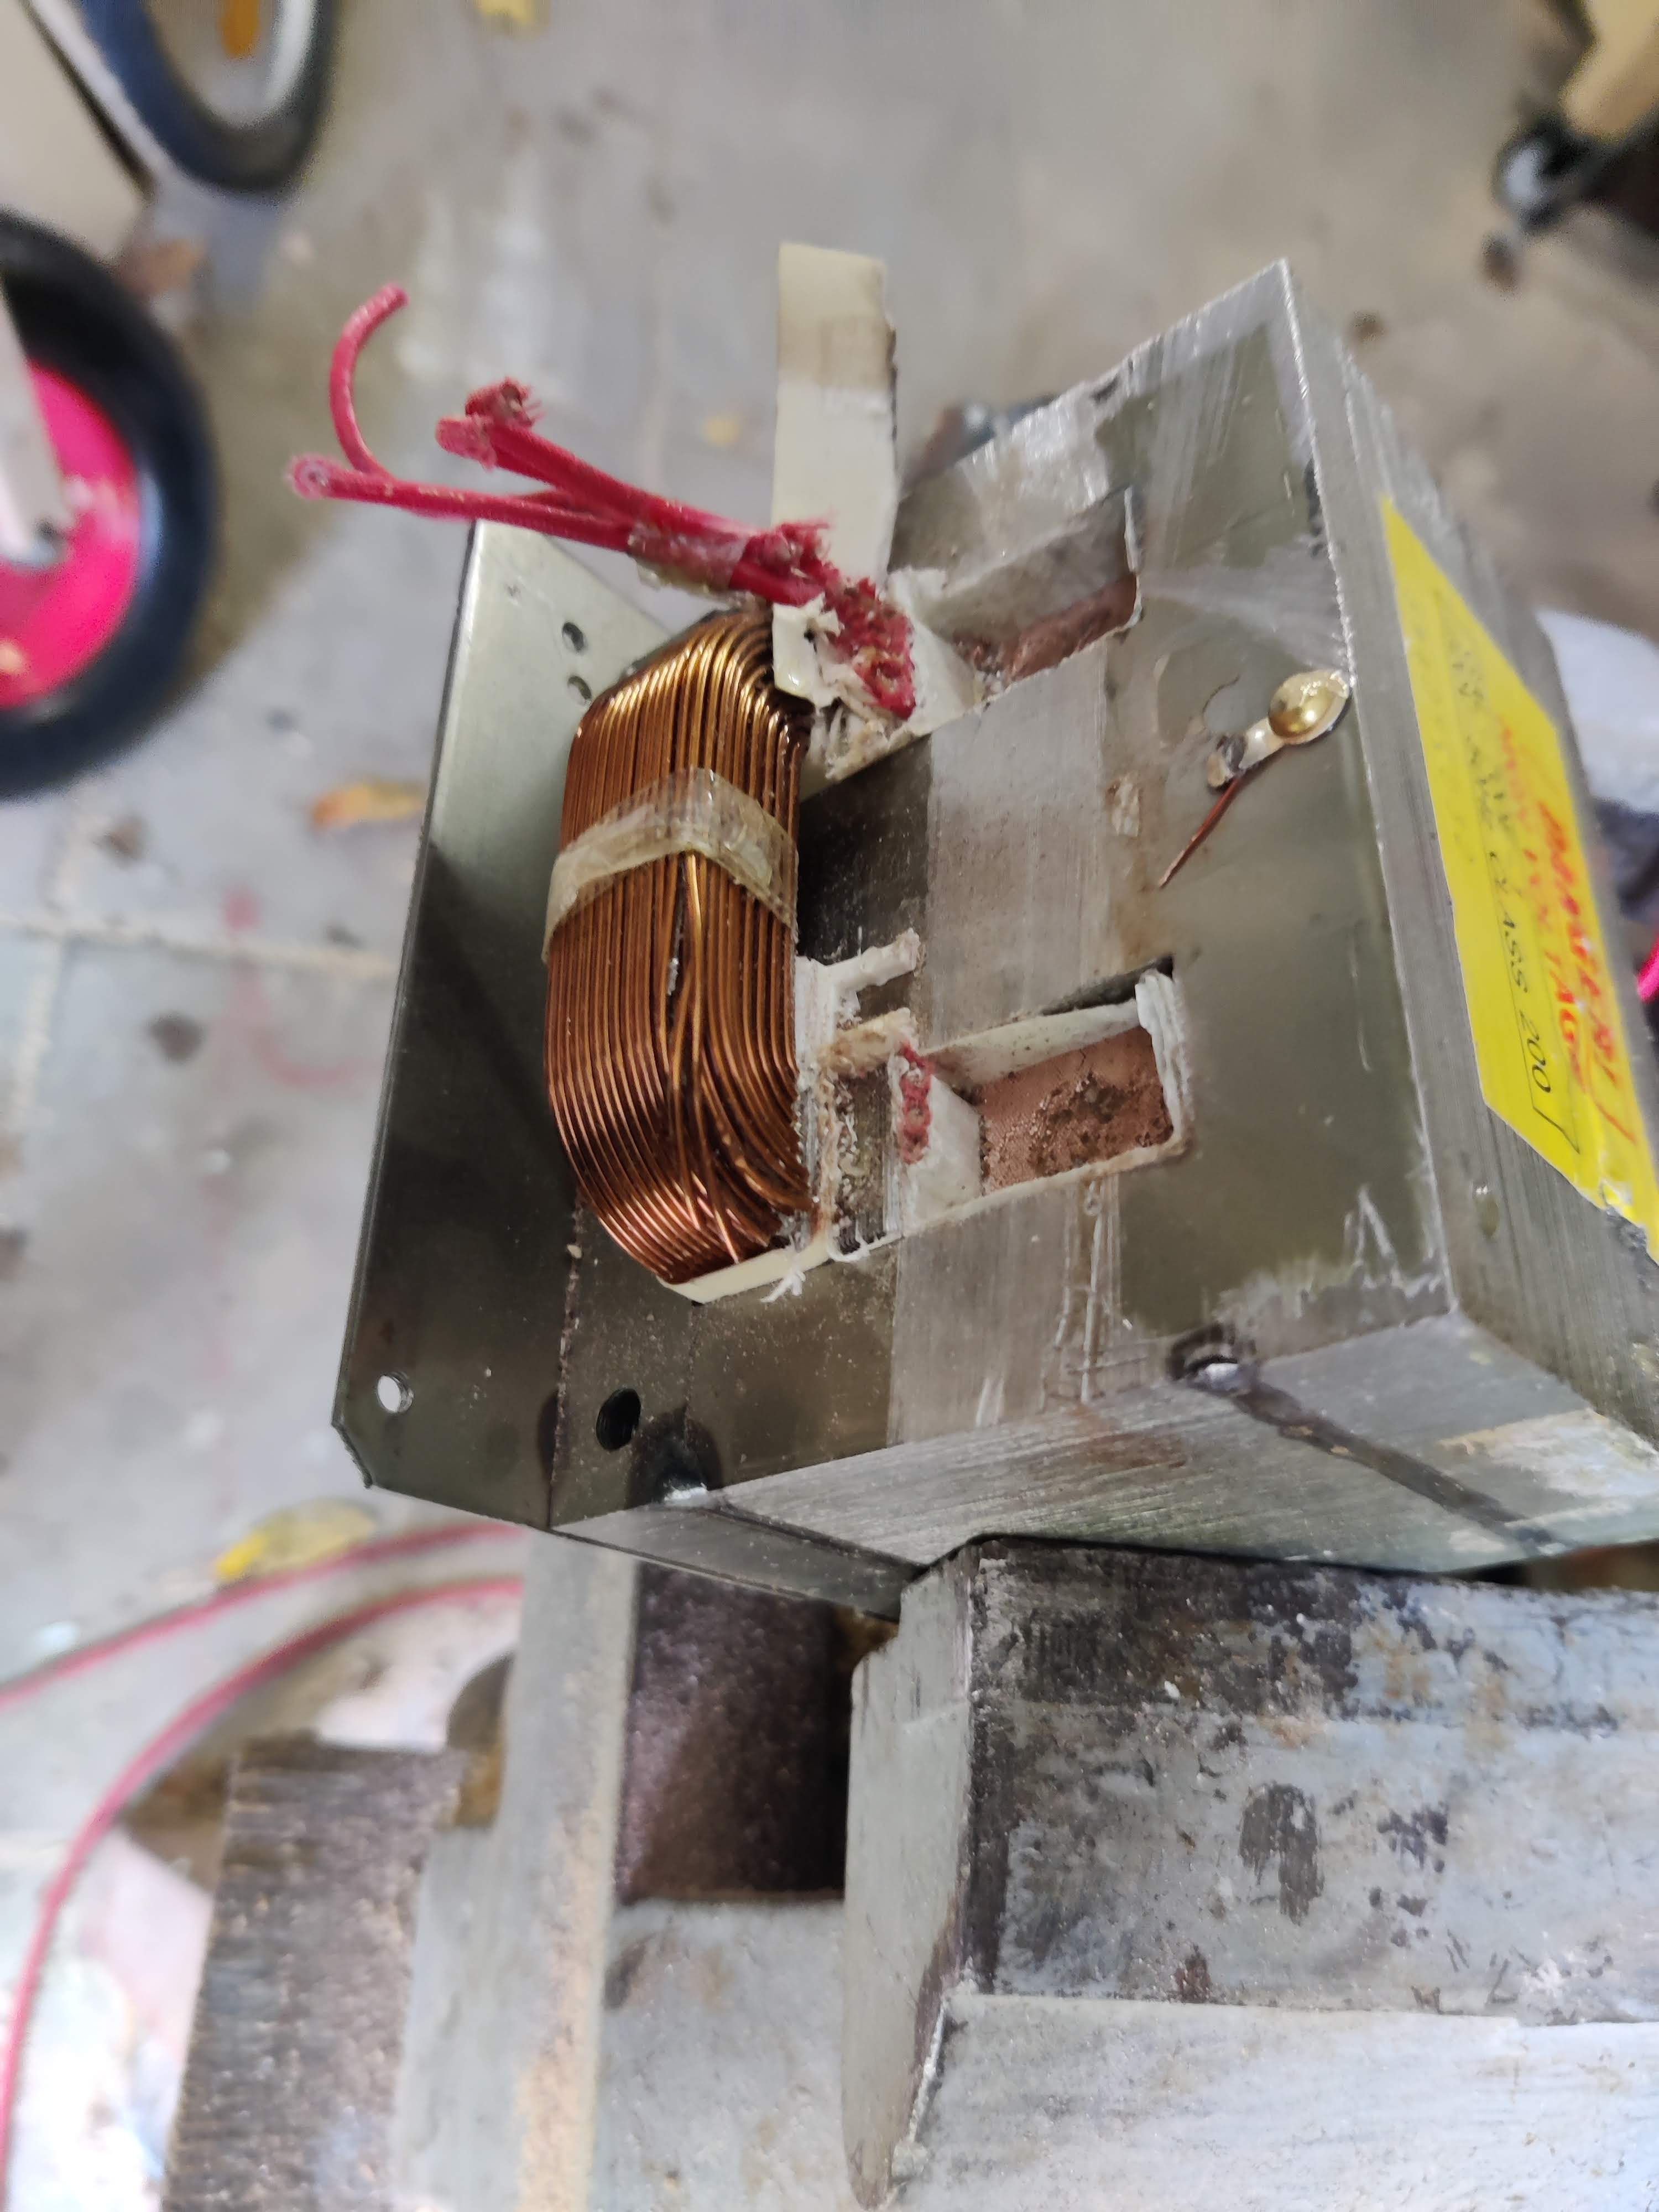
\includegraphics[width=10cm]{images/KaputterTransformator}
    \caption{Kaputter primärer Block\cite{lorenz_scherrer_selbst_2023}}
    \label{fig:35}
\end{figure}

\subsection*{Allgemeine Grundeinstellungen}\label{sec:parameter}
\begin{enumerate}[label=\arabic*.]
    \item Maximale Fahrgeschwindigkeit
    \item Rad-Durchmesser
    \item Metrische und imperiale Einheiten
\end{enumerate}

\section{P-Parameter-Einstellung}
\begin{enumerate}[label=\arabic*.]
    \item P1 Motorumdrehung Einstellung (Alnico-Zahl)
    \item P2 Geschwindigkeitssignal Einstellung
    \item P3 Motor Unterstützungsmodus
    \item P4 Daumengas Startmodus
    \item P5 Batterie - Ladezustandsanzeige
\end{enumerate}

\section{C-Parameter-Einstellung}
\begin{enumerate}[label=\arabic*.]
    \item C1 PAS - Sensor Parametereinstellung
    \item C2 Motor Phasen Anpassung
    \item C3 Einstellung der Anzahl der Unterstützungsstufen
    \item C4 Daumengas Funktionseinstellung
    \item C5-Controller maximale Stromeinstellung
    \item C6-Hintergrundbeleuchtung Helligkeitseinstellung
    \item C7 Cruise Funktionseinstellung
    \item C8 Motor Betriebstemperatur Anzeige
    \item C9 Power on Passwort Einstellung
    \item C10 Wiederherstellung Werkseinstellung
    \item C11 Einstellung Übertragungsprotokoll
    \item C12-Controller Unterspannungseinstellung
    \item C13 Bremsenergiegewinnung
    \item C14 Abstimmung der Unterstützungsstufen
\end{enumerate}

\begin{figure}[h]
    \centering
    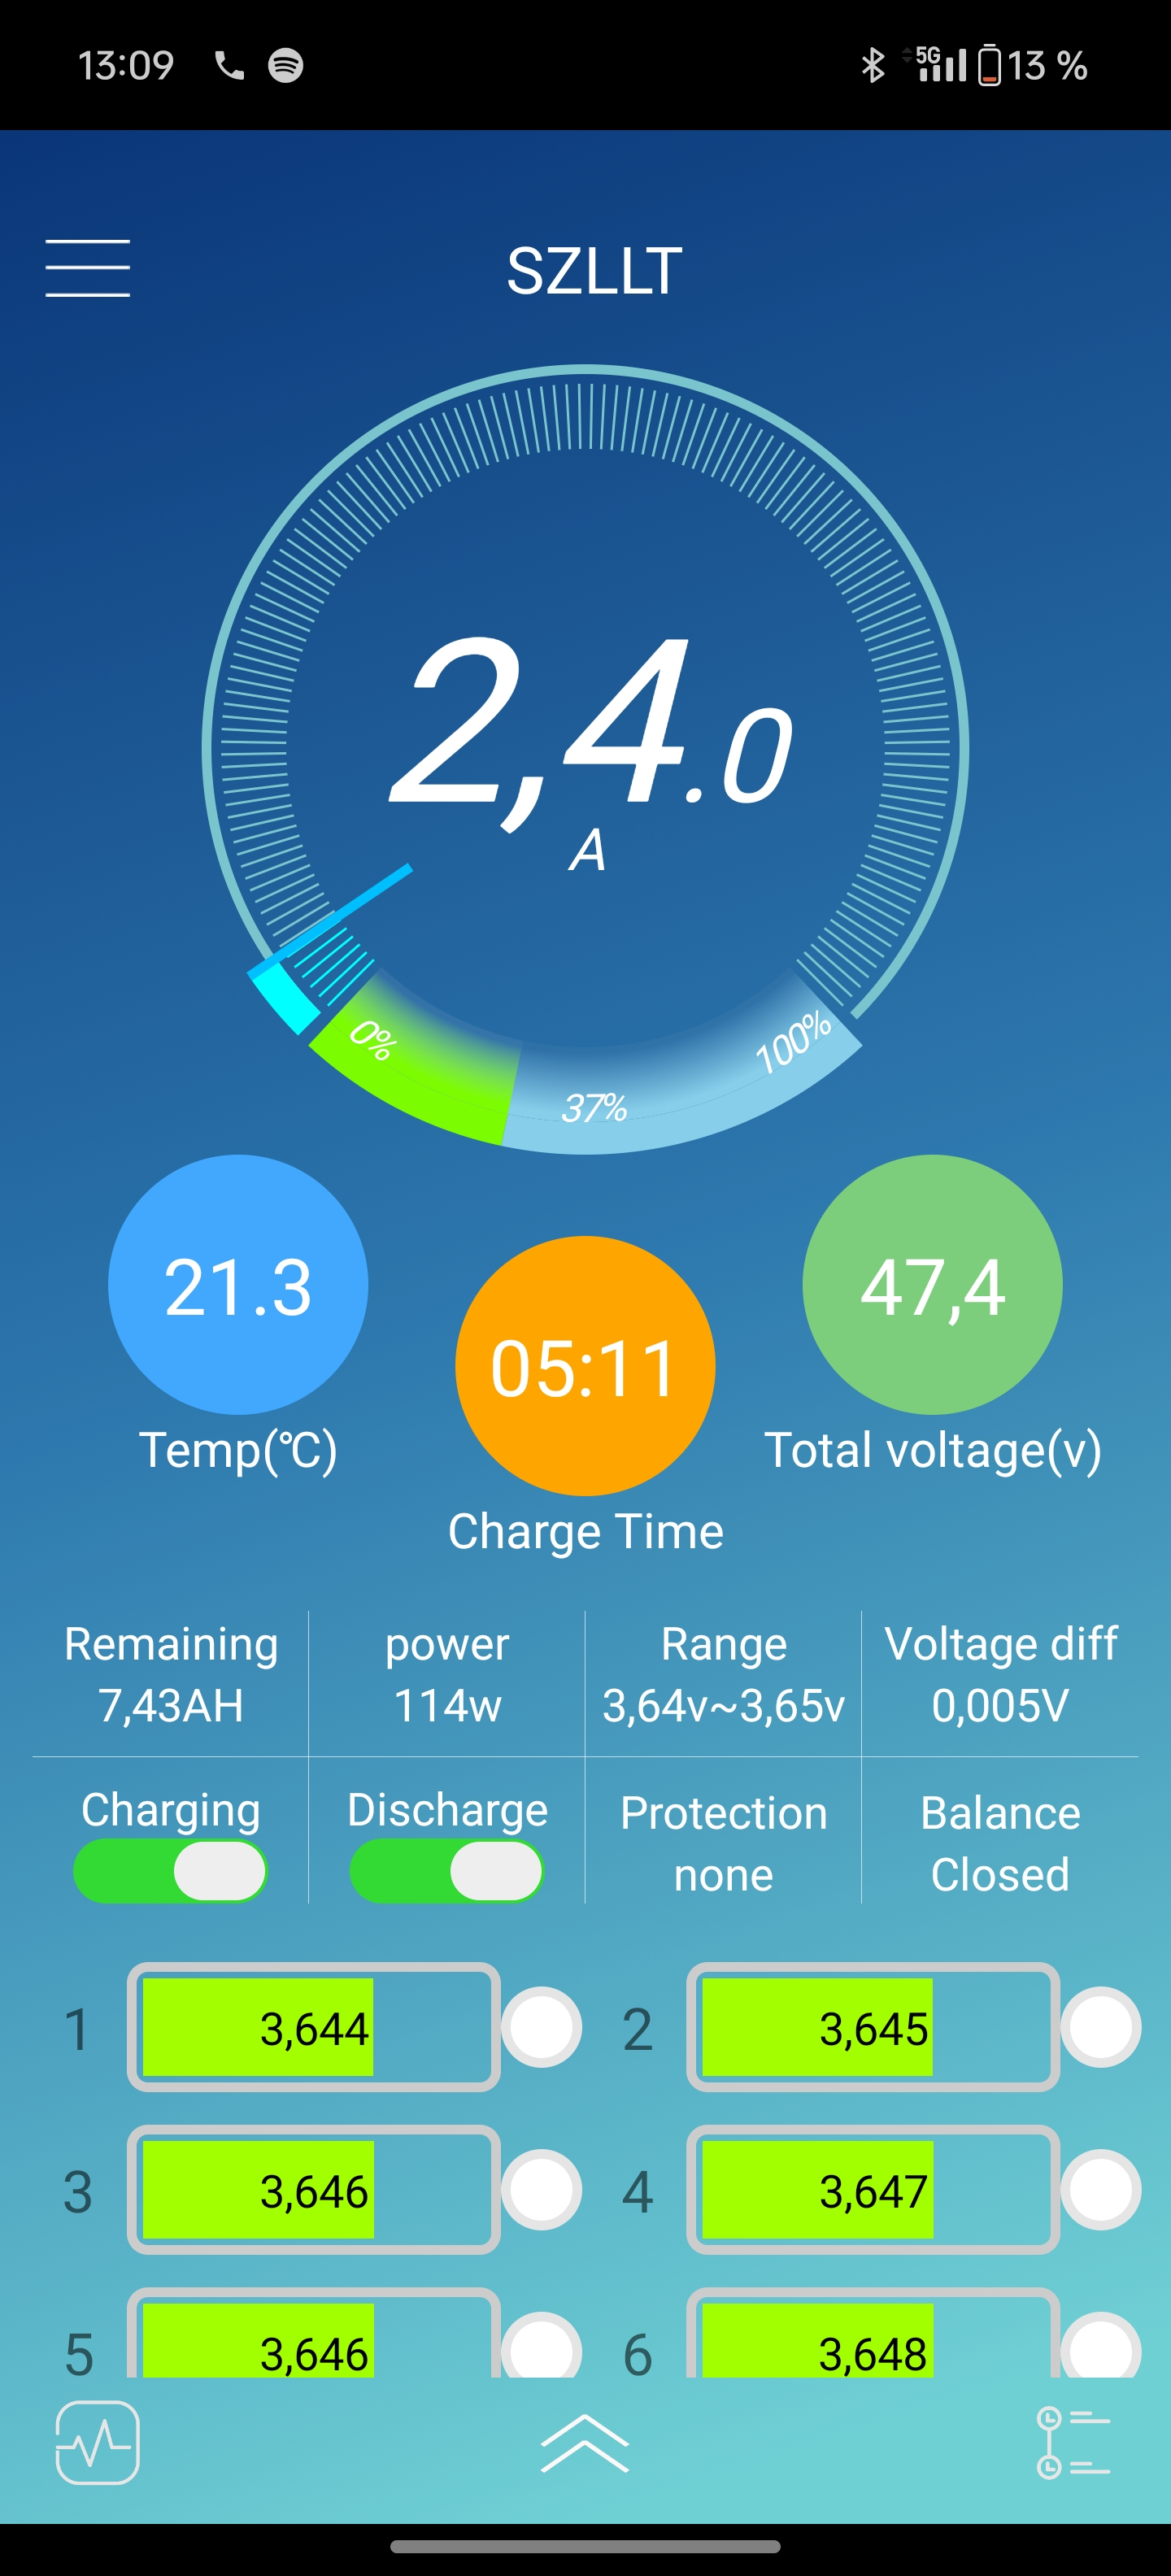
\includegraphics[width=10cm]{images/Batterie vor dem laden}
    \caption{Batteriestand vor dem Laden\cite{lorenz_scherrer_selbst_2023}}
    \label{fig:36}
\end{figure}

\begin{figure}[h]
    \centering
    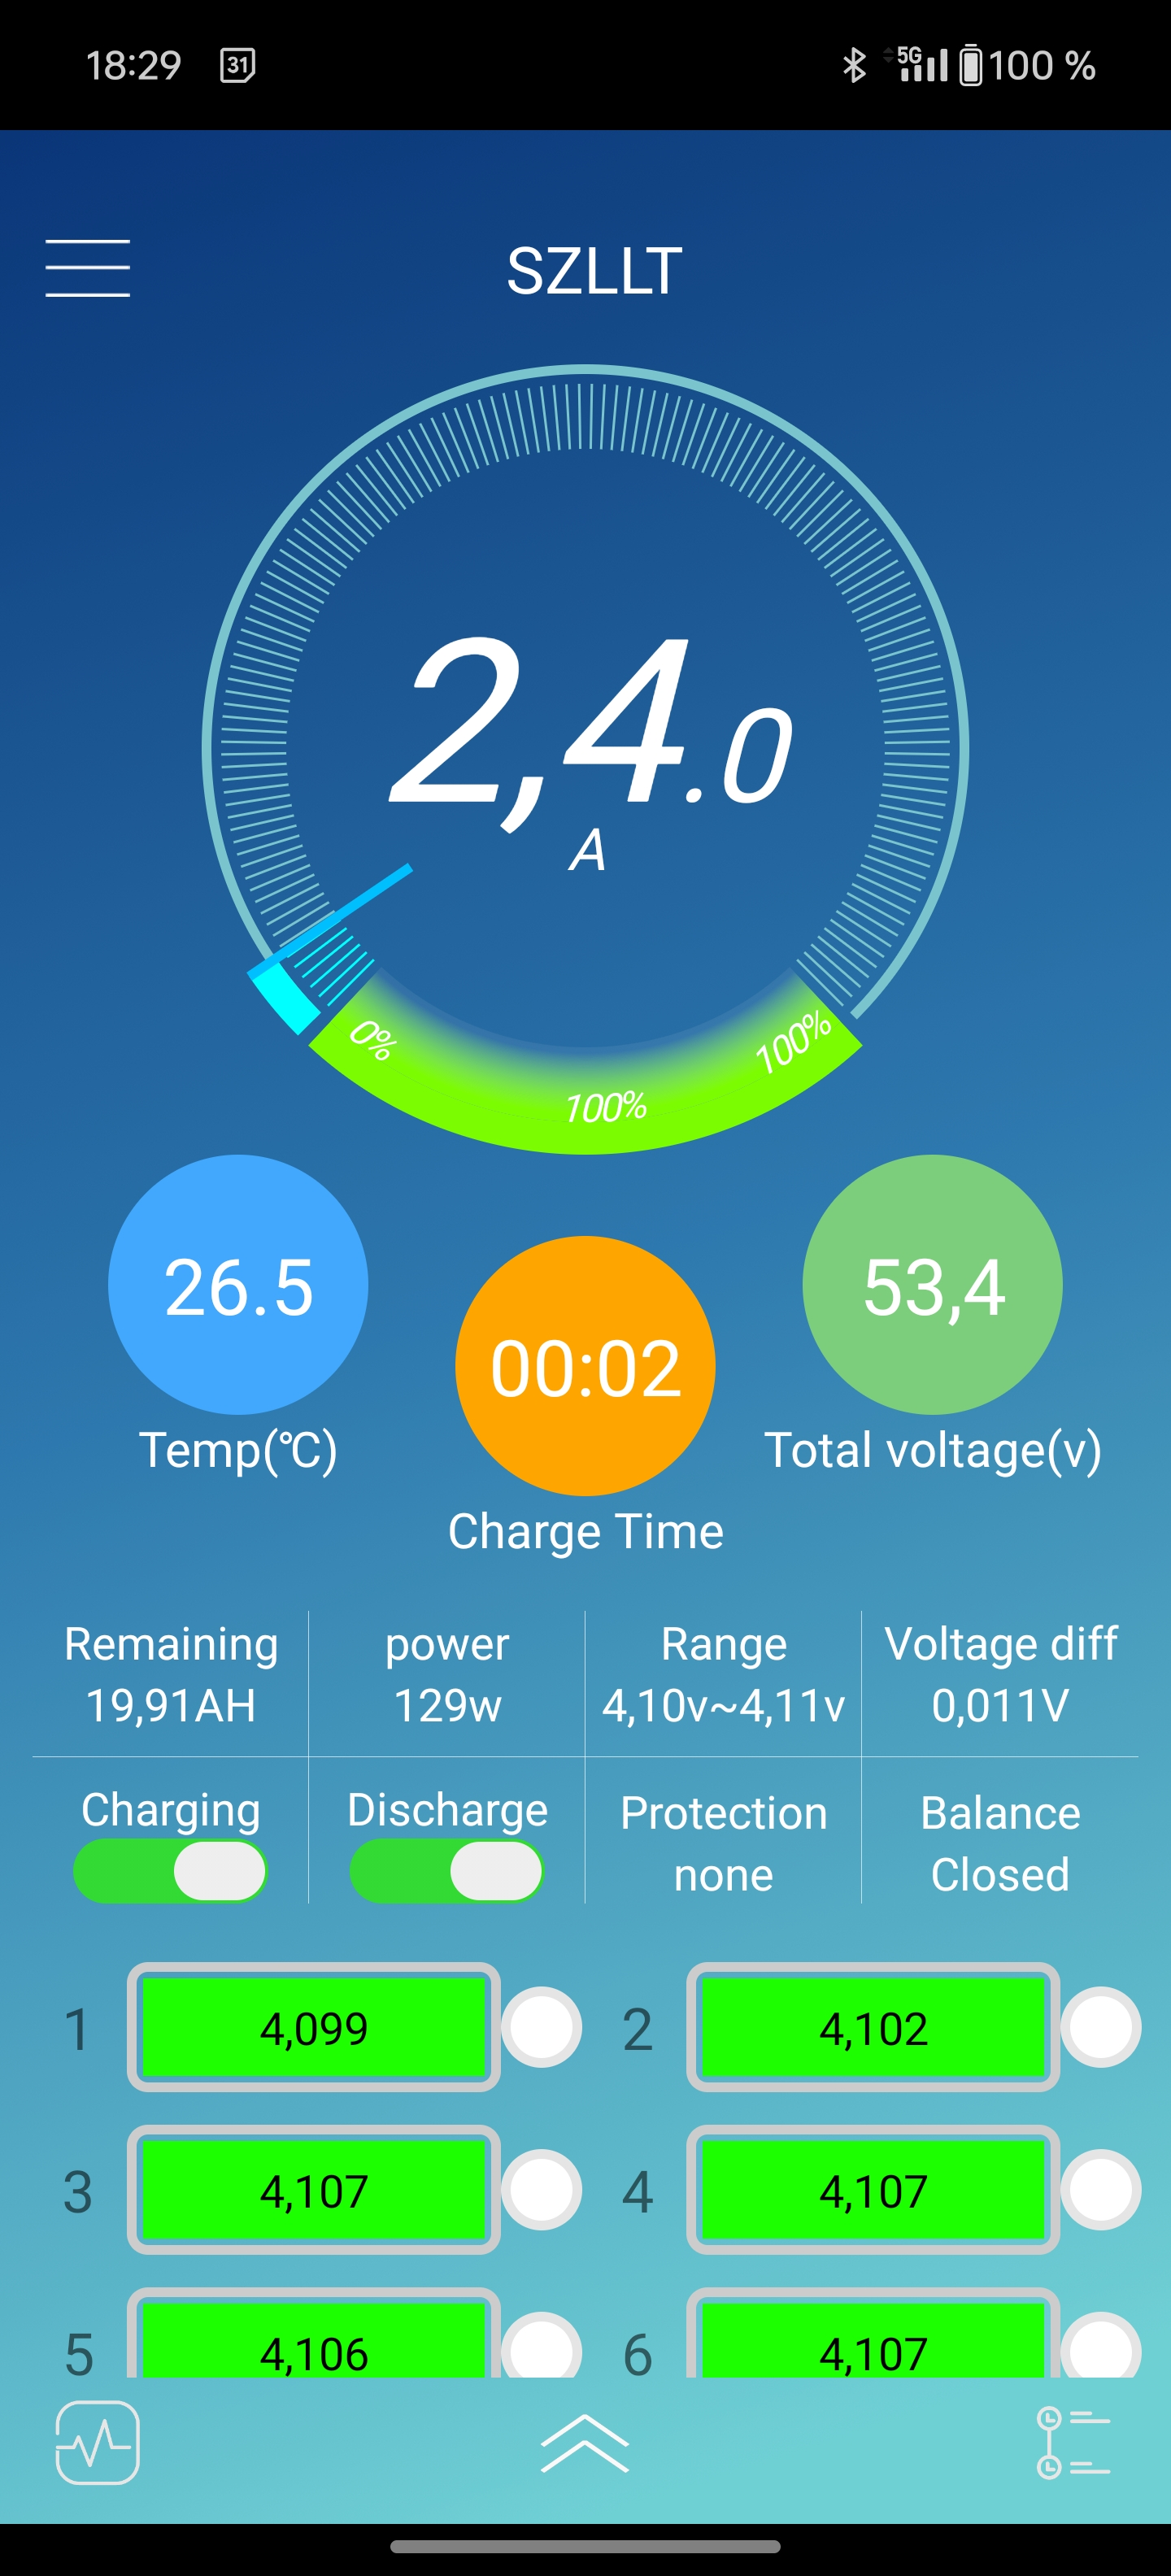
\includegraphics[width=10cm]{images/Batterienachdemladen}
    \caption{Batteriestand nach dem Laden\cite{lorenz_scherrer_selbst_2023}}
    \label{fig:37}
\end{figure}



